\documentclass[a4paper,12 pt]{article}

%% Language and font encodings
\usepackage[spanish,es-tabla]{babel}
\usepackage[utf8]{inputenc}
\usepackage[T1]{fontenc}
\usepackage{cite}
\usepackage{amsmath, amsthm, amssymb, amsfonts} 
\usepackage[mathscr]{eucal}
\usepackage{ulem} % subrayar, tachar
\usepackage{hyperref} % para el url
\usepackage{multirow, array} % para las tablas
\usepackage{float} % para tablas [H]
\usepackage{graphicx} % graficos
\usepackage{titlesec} %subsubsubsection
\usepackage[usenames]{color} %palabras con color
\usepackage{lscape} % texto horizontal
\usepackage{pdflscape} % hoja horizontal
\usepackage{booktabs} %tabla con puntos

\newcolumntype{P}[1]{>{\centering\arraybackslash}p{#1}}
\newcolumntype{M}[1]{>{\centering\arraybackslash}m{#1}}
\newcolumntype{L}[1]{>{\raggedleft\arraybackslash}p{#1}}
\newcolumntype{R}[1]{>{\raggedright\arraybackslash}p{#1}}
  
%counter
\newcounter{mycounter} % create a new counter, called 'mycounter'
% default def'n of '\themycounter' is '\arabic{mycounter}'

%% command to increment 'mycounter' by 1 and to display its value:
\newcommand\showmycounter{\stepcounter{mycounter}\themycounter}

\usepackage{lipsum}
\newcommand\showlips{\stepcounter{mycounter}\lipsum[\value{mycounter}]}


%% Sets page size and margins
\usepackage[a4paper,top=2cm,bottom=2cm,left=2cm,right=2cm,marginparwidth= 1.5cm]{geometry}
  
\title{\LARGE \textbf{\\[0.5cm] Ingenio\\[2.5cm]}}

% Chicos, porfavor incluyan sus nombres en orden alfabetico
\author{\textbf{Grupo 7}\\[0.5cm]
        Valeria Huepa Ducuara\\
        Juan José Peña Becerra\\
        Carlos Daniel Rincón Mora\\
        Guiselle Tatiana Zambrano Penagos\\[2.5cm]
        Sebastian David Moreno Bernal\\[2.5cm]}
\date{}

\begin{document}

\newpage

\begin{figure}
    \centering
    
\includegraphics[width=0.57\textwidth]{images/escudoUN.png}
\end{figure}
\maketitle 
\thispagestyle{empty}

\begin{center}
    \small Universidad Nacional de Colombia\\
    Facultad de Ingeniería\\
    Departamento de Ingeniería de Sistemas e Industrial\\
    Ingeniería de Sistemas\\
    Ingeniería de Software II\\
    Bogotá, Colombia\\
    2020
\end{center}
\newpage
\tableofcontents % indice de contenidos}
\thispagestyle{empty}

\newpage
\setcounter{page}{1}
\pagestyle{plain}

\section{Descripción General}


\subsection{Descripción del Problema}

Dada la existencia de una necesidad de tener una plataforma online, adicionalmente no
existen muchos canales de información para personas interesadas en el campo de la
Ingeniería que quieran mantenerse informadas diariamente por medio de informes,
artículos y noticias de parte de una fuente confiable y en constante actualización,
esto es porque los canales existentes no se mantienen en continuo mantenimiento o no
son de agrado para el público en mención. Así mismo, hoy en día circulan noticias
falsas por redes sociales, y en otros medios de comunicación quitando la certeza y
veracidad de la información. Se desea una plataforma más personal, en donde las
personas del campo de la Ingeniería pueden conocerse e interactuar entre ellas, para
obtener conocimiento en diversas áreas en común de interés para cada uno, además de
comentar a los demás usuarios su opinión de cierto tema.\\

\subsection{Descripción del Producto}

El software a realizar pretende tener un vínculo con el público interesado en temas
actuales de Ingeniería (Stakeholders), y desea brindarle información de primera mano,
así como artículos (científicos, de opinión y periodísticos ) de gran interés para el
mundo actual, con autores de renombre en la industria de Ingeniería. Así mismo, podrán
registrarse para recibir notificaciones cada que algún artículo de su posible interés
sea publicado. Recibirán notificaciones de sus autores preferidos, para mantenerse
actualizados con el trabajo de reconocidos ingenieros.\\

Se desea realizar una plataforma más personal, que las que existen actualmente, en la
cual los usuarios puedan conocer a otras personas con intereses similares en el campo
de la Ingeniería, además de conocer, seguir y comentar el trabajo de otros ingenieros.
El registro como usuario es de carácter público, mientras que para que para ser autor y
poder realizar una publicación, esté debe ser aprobado por el administrador,
demostrando conocimiento en un área de interés, presentado comprobantes de estudios y
experiencia académica o laboral.\\

La plataforma cuenta con diferentes foros, en los cuales los usuarios podrán dar su
opinión de forma libre, siempre y cuando sean respetuosos con los demás usuarios y
autores, en caso contrario su cuenta podría ser vetada o eliminada de la plataforma.

% arreglar: Mejorar la descripción de los roles
\subsection{Descripción de los Roles de Usuario}

\begin{itemize}
    \item \textbf{Administrador:} Individuo que posee el rol de usuario y administrador,
    este tiene permisos especiales que le permiten otorgar o despojar el rol de autor
    para los usuarios, este tendrá que verificar que el usuario que desee publicar
    contenido en la plataforma posea comprobantes que respalden su experiencia académica
    y laboral sobre uno o varios temas relacionados con la ingeniería, también será el
    responsable de atender las diferentes denuncias realizadas por los usuarios y
    determinar si es pertinente o no vetar o eliminar al usuario denunciado.
    
    \item \textbf{Autor:} Individuo que posee el rol de usuario y autor, este puede 
    publicar contenido relacionado con la ingeniería en la plataforma e interactuar
    con los demás usuarios, para publicar información este puede hacerlo en formato
    PDF, JPG o PNG, podrá agregar archivos de opinión, investigación y noticias
    clasificándolos en una o mas categorías (computación, electrónica y robótica)
    y presentar esta información por medio de infografías, o texto plano.
    
    \item \textbf{Usuario:} Es el rol que tendrán todos los individuos que se
    registren en la plataforma, este podrá suscribirse a una o más categorías lo que
    le permitirá tener una sección de cada una en la pantalla de inicio, con los
    diferentes archivos pertenecientes a esta. Este también podrá seguir a autores y
    otros usuarios y recibir notificaciones cada vez que estos publiquen archivos de
    información o realicen comentarios en los foros. Este usuario podrá acceder a la
    información de la plataforma por medio de un buscador general (filtrando por
    palabras clave) o especializada (fecha de publicación, autor, categoría y tipo).
    
    \item \textbf{Visitante:} Este podrá ver la pagina principal de noticias y
    acceder al buscador general (filtrando por palabras clave), podrá ver las
    diferentes categorías y acceder a los artículos e infografías, más no podrá
    suscribirse a ninguna categoría, seguir autores o usuarios ni comentar en ningún
    foro. Si este desea acceder a más funcionalidades, tendrá que registrarse a la
    plataforma.
\end{itemize}{}

\section{Descripción del Equipo y Metodología de Desarrollo}

La metodología a seguir en este proyecto es Scrum, siguiendo todas las etapas y
características de la metodología mencionada. El manejo del código de software se
manejará por medio de un sistema de control de versiones central, usando las
herramientas Git y GitHub por parte de cada uno de los desarrolladores. \\

Para el correcto avance del proyecto se realizarán entregas parciales con análisis de
cada aspecto de este. Las fechas de los avances del proyecto serán de la siguiente
manera:

\begin{itemize}
    \item \textbf{Iteración 0:} Marzo 24 del 2020
    \item \textbf{Iteración 1:} Abril 14 del 2020
    \item \textbf{Iteración 2:} Mayo 5 del 2020
    \item \textbf{Iteración 3:} Mayo 26 del 2020
    \item \textbf{Iteración 4:} Junio 16 del 2020
    \item \textbf{Iteración Final:} Junio 23 del 2020
\end{itemize}{}

\subsection{Roles del equipo}

La forma en la que se trabajará durante el desarrollo del software será en equipos de 2
personas, donde uno de ellos trabajará en el front-end y otro en el back-end, los
equipos serán redefinidos en cada iteración y estos mantendrán comunicación diaria,
mientras que los reportes de avances por equipo serán realizados 2 veces por semana,
donde todos los desarrolladores estarán presentes.

\begin{table}[H]
    \centering
    \small{
    \begin{tabular}{|c|c|}
        \hline
        \textbf{Rol}   &   \textbf{Nombre}  \\ 
        \hline
        Product Owner   &   Sebastian David Moreno Bernal\\
        \hline
        Scrum Master   &   Guiselle Tatiana Zambrano Penagos\\
        \hline
        \multirow{2}{2cm}{Front End}    &   Valeria Huepa Ducuara\\
            &   Carlos Daniel Rincón Mora\\
        \hline
        \multirow{2}{2cm}{Back End}    &   Juan José Peña Becerra\\
            &   Guiselle Tatiana Zambrano Penagos\\
        \hline
         
    \end{tabular}
    \caption{Roles del equipo}}
    \label{T00}
\end{table}{}

\subsection{Recursos del equipo}

\begin{table}[H]
    \centering
    \small{
    \begin{tabular}{|M{2cm}|M{1.5cm}|M{3cm}|M{3cm}|M{1.5cm}|M{2cm}|}
        \hline
        \textbf{Nombre}    &\textbf{Marca}     &\textbf{Sistema Operativo} 
        &\textbf{Procesador}   &\textbf{RAM}   &\textbf{Capacidad}\\
        \hline
        Valeria Huepa                       &Asus   &Windows 10 Home x64 
        & Intel(R) Core(TM) i5-4210U CPU    &12GB   &HDD 240GB \\
        \hline
        Juan Peña                           &Asus   &Windows 10 Home x64
        &Intel(R) Core(TM) i5-6198DU CPU @ 2.30 GHz &8GB    &HDD 240GB\\
        \hline
        Carlos Rincón                       &Asus   &Windows 10 Home x64
        &Intel(R) Core(TM) i7-3537U CPU @ 2.00GHz   &8GB    &SSD 128GB\\
        \hline
        Tatiana Zambrano                    &Lenovo &Kali Linux x64
        &AMD A8 - 7410 2.2 GHz              &4GB    &HDD 500GB\\
        \hline
    \end{tabular}
    \caption{Recursos del equipo}
    \label{T01}}
\end{table}{}

% arreglar: Completar info
\subsection{Disposición del equipo}

% nombre, frecuencia semanal (días por se, horas de desarrollo diario
\begin{table}[H]
    \centering
    \small{
    \begin{tabular}{|M{2cm}|M{4cm}|M{4cm}|}
        \hline
        \textbf{Nombre}    & \textbf{Frecuencia Semanal (días por semana)}   
        &\textbf{Horas de desarrollo por día}\\
        \hline
        Valeria Huepa   &       &       \\
        \hline
        Juan Peña       &       &       \\
        \hline
        Carlos Rincón   &   5    &  2     \\
        \hline
        Tatiana Zambrano    & 5      &  2     \\
        \hline
    \end{tabular}
    \caption{Caption}
    \label{tab:my_label}}
\end{table}{}

\section{Historias de Usuario}

Para la elaboración de las historias de usuarios se definieron diferentes criterios de
riesgo y prioridad, que facilitará la clasificación de cada historia en estas
categorías, y al mismo tiempo, determinar cuál de ellas elaborar primero y la atención
requerida en las dependencias y el manejo de datos a las que estas tiene acceso.\\

Para determinar el nivel de esfuerzo requerido en la elaboración de las historias (donde
este este no está relacionado con el tiempo invertido en ellas), fue utilizada la
técnica planning poker, donde tomamos como historia base la "creación de una cuenta" por
parte del rol \textit{visitante}, a la que le fue asignada un esfuerzo de 3 puntos. El
esfuerzo de las otras historias fue determinado por un consenso grupal en donde se
comparaba la complejidad de las historias faltantes con la historia base.\\

\begin{table}[H]
    \centering
    \small{
    \begin{tabular}{|M{1cm}|M{2cm}|M{11cm}|}
        \hline
        \textbf{Valor}   &\textbf{Significado}   &\textbf{Criterio}\\
        \hline 
        \multirow{1}{1cm}{\centering 1}    
            &\multirow{1}{2cm}{\centering Muy bajo}
            & La historia describe una funcionalidad que no soluciona ninguna parte del
            problema propuesto, ni otras historias dependen de esta para su correcto
            funcionamiento.    \\
        \hline
        \multirow{1}{1cm}{\centering 2}    
            &\multirow{1}{2cm}{\centering Bajo}
            & La historia describe una funcionalidad relacionada con la solución de una
            parte del problema propuesto, pero esta no es indispensable para el correcto
            funcionamiento de la plataforma.  \\
        \hline
        \multirow{1}{1cm}{\centering 3}    
            &\multirow{1}{2cm}{\centering Moderado}
            & La historia describe una funcionalidad que resuelve una parte del problema
            propuesto y otras historias dependen poco de ella para su correcto
            funcionamiento. \\
        \hline
        \multirow{1}{1cm}{\centering 4}    
            &\multirow{1}{2cm}{\centering Alto}
            & La historia describe una funcionalidad que resuelve una parte del problema
            propuesto y otras historias dependen en gran medida de esta para su correcto
            funcionamiento.\\
        \hline
        \multirow{1}{1cm}{\centering 5}    
            &\multirow{1}{2cm}{\centering Muy alto}
            & La historia describe una funcionalidad que resuelve una parte del problema
            propuesto, otras historias dependen en gran medida de esta para su correcto
            funcionamiento o maneja datos sensibles de los usuarios de la plataforma.\\
        \hline
    \end{tabular}
    \caption{Niveles de riesgo}
    \label{Nriesgo}}
\end{table}{}

\begin{table}[H]
    \centering
    \small{
    \begin{tabular}{|M{1cm}|M{2cm}|M{11cm}|}
        \hline
        \textbf{Valor}   &\textbf{Significado}   &\textbf{Criterio}\\
        \hline 
        \multirow{1}{1cm}{\centering 1}    
            &\multirow{1}{2cm}{\centering Muy baja}
            & La historia no formula una funcionalidad que solucione alguna parte del
            problema propuesto. \\
        \hline
        \multirow{1}{1cm}{\centering 2}    
            &\multirow{1}{2cm}{\centering Baja}
            & La historia formula una funcionalidad que está relacionada con la solución
            de alguna parte del problema propuesto.\\
        \hline
        \multirow{1}{1cm}{\centering 3}    
            &\multirow{1}{2cm}{\centering Moderada}
            & La historia describe una funcionalidad que soluciona una parte del
            problema propuesto pero esta no es crítica u otras historias no dependen 
            de esta para su elaboración. \\
        \hline
        \multirow{1}{1cm}{\centering 4}    
            &\multirow{1}{2cm}{\centering Alta}
            & La historia describe una funcionalidad que soluciona una parte del
            problema propuesto y otras historias dependen de esta para ser elaboradas.\\
        \hline
        \multirow{1}{1cm}{\centering 5}    
            &\multirow{1}{2cm}{\centering Muy alta}
            & La historia describe una funcionalidad que soluciona una parte crítica del
            problema propuesto y debe ser realizada en el menor tiempo posible.\\
        \hline
    \end{tabular}
    \caption{Niveles de prioridad}
    \label{Nprioridad}}
\end{table}{}


\subsection{Rol-Visitante}

% PLANTILLA PARA VISITANTE
\begin{table}[H]
    \centering
    \small{
    \begin{tabular}{|M{3.5cm}|M{3.5cm}|M{3.5cm}|M{3.5cm}|}
        \hline
        \multicolumn{4}{|c|}{\textbf{Buscar contenido (titulo, palabras)}}\\
        \hline
        \textbf{ID} &\showmycounter &\textbf{Rol}                   &  Visitante \\
        \hline
        \textbf{Prioridad}       &  5 &\textbf{Riesgo en Desarrollo}  &  5 \\
        \hline
        \textbf{Puntos Esfuerzo}    & 4  &\textbf{Iteración Asignada}    &  1 \\
        \hline
        \multirow{2}{3cm}{\centering\textbf{Programadores asignados}} 
            &\multicolumn{3}{|c|}{ Front: H. Valeria }\\
            &\multicolumn{3}{|c|}{ Back: P. Juan}\\
        \hline
        \multirow{4}{3cm}{\centering\textbf{Descripción}}
            &\multicolumn{3}{|p{12cm}|}{
                \textcolor{red}{Como} Visitante
            }\\
            &\multicolumn{3}{|p{12cm}|}{
                \textcolor{red}{Quiero} Buscar el contenido disponible en el sitio web (por titulo o palabras en el titulo)
            }\\
            &\multicolumn{3}{|p{12cm}|}{
                \textcolor{red}{Con el fin de} ver parte del contenido del sitio web
            }\\
        \hline
        \multirow{2}{3cm}{\centering\textbf{Validación}}
            & \multicolumn{3}{|p{12cm}|}{
                Cada visitante podrá ver una lista en que aparezcan los resultados de su búsqueda
            }\\
        \hline
    \end{tabular}
    \caption{Buscar Contenido}
    \label{Visit00}}
\end{table}{}

\begin{table}[H]
    \centering
    \small{
    \begin{tabular}{|M{3.5cm}|M{3.5cm}|M{3.5cm}|M{3.5cm}|}
        \hline
        \multicolumn{4}{|c|}{\textbf{Acceder a la publicación}}\\
        \hline
        \textbf{ID} &\showmycounter &\textbf{Rol}                   &  Visitante \\
        \hline
        \textbf{Prioridad}       &  5 &\textbf{Riesgo en Desarrollo}  &  5 \\
        \hline
        \textbf{Puntos Esfuerzo}    & 3  &\textbf{Iteración Asignada}    &  2 \\
        \hline
        \multirow{2}{3cm}{\centering\textbf{Programadores asignados}} 
            &\multicolumn{3}{|c|}{ Front: R. Carlos }\\
            &\multicolumn{3}{|c|}{ Back: P. Juan}\\
        \hline
        \multirow{4}{3cm}{\centering\textbf{Descripción}}
            &\multicolumn{3}{|p{12cm}|}{
                \textcolor{red}{Como} Visitante
            }\\
            &\multicolumn{3}{|p{12cm}|}{
                \textcolor{red}{Quiero} acceder a una publicación.
            }\\
            &\multicolumn{3}{|p{12cm}|}{
                \textcolor{red}{Con el fin de}  Ver información de la publicación (texto,imágenes, noticias) desde el sitio web.
            }\\
        \hline
        \multirow{1}{3cm}{\centering\textbf{Validación}}
            & \multicolumn{3}{|p{12cm}|}{
                Cada visitante podrá ver una lista en que aparezcan los resultados de su búsqueda
            }\\
        \hline
    \end{tabular}
    \caption{Acceder a publicación}
    \label{Visit01}}
\end{table}{}

\begin{table}[H]
    \centering
    \small{
    \begin{tabular}{|M{3.5cm}|M{3.5cm}|M{3.5cm}|M{3.5cm}|}
        \hline
        \multicolumn{4}{|c|}{\textbf{Creación de cuenta}}\\
        \hline
        \textbf{ID} &\showmycounter &\textbf{Rol}                   &  Visitante \\
        \hline
        \textbf{Prioridad}       &  4 &\textbf{Riesgo en Desarrollo}  &  3 \\
        \hline
        \textbf{Puntos Esfuerzo}    & 3  &\textbf{Iteración Asignada}    &  1 \\
        \hline
        \multirow{2}{3cm}{\centering\textbf{Programadores asignados}} 
            &\multicolumn{3}{|c|}{ Front: R. Carlos }\\
            &\multicolumn{3}{|c|}{ Back: Z. Tatiana}\\
        \hline
        \multirow{4}{3cm}{\centering\textbf{Descripción}}
            &\multicolumn{3}{|p{12cm}|}{
                \textcolor{red}{Como} Visitante
            }\\
            &\multicolumn{3}{|p{12cm}|}{
                \textcolor{red}{Quiero} Crear un usuario en el sistema
            }\\
            &\multicolumn{3}{|p{12cm}|}{
                \textcolor{red}{Con el fin de}  acceder al sistema  para hacer uso de funcionalidades.
            }\\
        \hline
        \multirow{1}{3cm}{\centering\textbf{Validación}}
            & \multicolumn{3}{|p{12cm}|}{
                Debe ingresar nombre, correo y contraseña
                La base de datos debe ser actualizada
                    Debe desplegarse un mensaje de confirmación

            }\\
        \hline
    \end{tabular}
    \caption{Creación de cuenta}
    \label{Visit02}}
\end{table}{}
%borrar
\subsection{Rol-Usuario}

% PLANTILLA PARA USUARIO

%1
\begin{table}[H]
    \centering
    \small{
    \begin{tabular}{|M{3.5cm}|M{3.5cm}|M{3.5cm}|M{3.5cm}|}
        \hline
        \multicolumn{4}{|c|}{\textbf{Inicio de sesión}}\\
        \hline
        \textbf{ID} &\showmycounter &\textbf{Rol}                       &  Usuario \\
        \hline
        \textbf{Prioridad}          & 5  &\textbf{Riesgo en Desarrollo}  &  4 \\
        \hline
        \textbf{Puntos Esfuerzo}    &  2 &\textbf{Iteración Asignada}    &  1 \\
        \hline
        \multirow{2}{3cm}{\centering\textbf{Programadores asignados}} 
            &\multicolumn{3}{|c|}{ H. Valeria }\\
            &\multicolumn{3}{|c|}{ Z. Tatiana}\\
        \hline
        \multirow{4}{3cm}{\centering\textbf{Descripción}}
            &\multicolumn{3}{|p{12cm}|}{
                \textcolor{red}{Como} Usuario
            }\\
            &\multicolumn{3}{|p{12cm}|}{
                \textcolor{red}{Quiero} iniciar sesión en el sistema.
            }\\
            &\multicolumn{3}{|p{12cm}|}{
                \textcolor{red}{Con el fin de} hacer uso de las funcionalidades a
                las que puedo acceder.
            }\\
        \hline
        \multirow{3}{3cm}{\centering\textbf{Validación}}
            & \multicolumn{3}{|p{12cm}|}{
                El usuario será redirigido a la página principal, donde podrá ver
                la sección de noticias general, los buscadores y las secciones de
                cada categoría a las que está suscrito.
            }\\
        \hline
    \end{tabular}
    \caption{Inicio de sesión para el rol usuario}
    \label{User01}}
\end{table}{}
%2
\begin{table}[H]
    \centering
    \small{
    \begin{tabular}{|M{3.5cm}|M{3.5cm}|M{3.5cm}|M{3.5cm}|}
        \hline
        \multicolumn{4}{|c|}{\textbf{Ver la información de mi cuenta}}\\
        \hline
        \textbf{ID} &\showmycounter &\textbf{Rol}                   &  Usuario \\
        \hline
        \textbf{Prioridad}          &  4 &\textbf{Riesgo en Desarrollo}  &  4 \\
        \hline
        \textbf{Puntos Esfuerzo}    &  2 &\textbf{Iteración Asignada}    &   1\\
        \hline
        \multirow{2}{3cm}{\centering\textbf{Programadores asignados}} 
            &\multicolumn{3}{|c|}{ R. Carlos }\\
            &\multicolumn{3}{|c|}{ P. Juan}\\
        \hline
        \multirow{5}{3cm}{\centering\textbf{Descripción}}
            &\multicolumn{3}{|p{12cm}|}{
                \textcolor{red}{Como} Usuario
            }\\
            &\multicolumn{3}{|p{12cm}|}{
                \textcolor{red}{Quiero} ver mi perfil 
            }\\
            &\multicolumn{3}{|p{12cm}|}{
                \textcolor{red}{Con el fin de} revisar mis datos personales, las
                categorías a las que estoy suscrito, la cantidad de usuarios que sigo o
                me siguen y ver cuántos y cuales publicaciones he guardado.
            }\\
        \hline
        \multirow{3}{3cm}{\centering\textbf{Validación}}
            & \multicolumn{3}{|p{12cm}|}{
                El usuario podrá acceder a una sección en donde podrá visualizar
                sus datos personales y los relacionados a este, que formen parte de la
                plataforma.
            }\\
        \hline
    \end{tabular}
    \caption{Ver información de la cuenta para el rol usuario}
    \label{User02}}
\end{table}{}
%3
\begin{table}[H]
    \centering
    \small{
    \begin{tabular}{|M{3.5cm}|M{3.5cm}|M{3.5cm}|M{3.5cm}|}
        \hline
        \multicolumn{4}{|c|}{\textbf{Modificar los datos de mi cuenta}}\\
        \hline
        \textbf{ID} &\showmycounter &\textbf{Rol}                   &  Usuario \\
        \hline
        \textbf{Prioridad}         & 5  &\textbf{Riesgo en Desarrollo}  &  5 \\
        \hline
        \textbf{Puntos Esfuerzo}    &  5 &\textbf{Iteración Asignada}    &  2 \\
        \hline
        \multirow{2}{3cm}{\centering\textbf{Programadores asignados}} 
            &\multicolumn{3}{|c|}{ R. Carlos }\\
            &\multicolumn{3}{|c|}{ P. Juan}\\
        \hline
        \multirow{3}{3cm}{\centering\textbf{Descripción}}
            &\multicolumn{3}{|p{12cm}|}{
                \textcolor{red}{Como} Usuario
            }\\
            &\multicolumn{3}{|p{12cm}|}{
                \textcolor{red}{Quiero} modificar mis datos personales
            }\\
            &\multicolumn{3}{|p{12cm}|}{
                \textcolor{red}{Con el fin de} actualizar o corregir mi información
                básica.
            }\\
        \hline
        \multirow{4}{3cm}{\centering\textbf{Validación}}
            & \multicolumn{3}{|p{12cm}|}{
               El usuario será redirigido a un formulario en el que se le permitirá
               ingresar su información nuevamente.
               Luego de guardar los cambios, el usuario será redirigido a su perfil en
               donde podrá verificar las modificaciones realizadas.
            }\\
        \hline
    \end{tabular}
    \caption{Modificar información de la cuenta para el rol usuario}
    \label{User03}}
\end{table}{}
%4
\begin{table}[H]
    \centering
    \small{
    \begin{tabular}{|M{3.5cm}|M{3.5cm}|M{3.5cm}|M{3.5cm}|}
        \hline
        \multicolumn{4}{|c|}{\textbf{Eliminar mi cuenta}}\\
        \hline
        \textbf{ID} &\showmycounter &\textbf{Rol}                   &  Usuario \\
        \hline
        \textbf{Prioridad}          & 3  &\textbf{Riesgo en Desarrollo}  & 4  \\
        \hline
        \textbf{Puntos Esfuerzo}    & 3  &\textbf{Iteración Asignada}    &  3 \\
        \hline
        \multirow{2}{3cm}{\centering\textbf{Programadores asignados}} 
            &\multicolumn{3}{|c|}{ Front: H. Valeria }\\
            &\multicolumn{3}{|c|}{ Back: Z. Tatiana}\\
        \hline
        \multirow{3}{3cm}{\centering\textbf{Descripción}}
            &\multicolumn{3}{|p{12cm}|}{
                \textcolor{red}{Como} Usuario
            }\\
            &\multicolumn{3}{|p{12cm}|}{
                \textcolor{red}{Quiero} eliminar mi cuenta.
            }\\
            &\multicolumn{3}{|p{12cm}|}{
                \textcolor{red}{Con el fin de} borrar toda información relacionada a mi
                usuario y no hacer parte de la revista.
            }\\
        \hline
        \multirow{6}{3cm}{\centering\textbf{Validación}}
            & \multicolumn{3}{|p{12cm}|}{
                El usuario podrá acceder a una opción desde su cuenta, que le permita
                eliminarla, al seleccionar dicha opción se le pedirá una validación y
                al ser aceptada el usuario será borrado y eliminado del sistema, por lo
                que su correo ya no será valido para ingresar a la plataforma y los
                demás usuarios no podrán ver la información relacionada a este.
            }\\
        \hline
    \end{tabular}
    \caption{Eliminar cuenta para el rol usuario}
    \label{User04}}
\end{table}{}
%5
\begin{table}[H]
    \centering
    \small{
    \begin{tabular}{|M{3.5cm}|M{3.5cm}|M{3.5cm}|M{3.5cm}|}
        \hline
        \multicolumn{4}{|c|}{\textbf{Realizar una búsqueda básica}}\\
        \hline
        \textbf{ID} &\showmycounter &\textbf{Rol}                   &  Usuario \\
        \hline
        \textbf{Prioridad}          & 5  &\textbf{Riesgo en Desarrollo}  &  4 \\
        \hline
        \textbf{Puntos Esfuerzo}    & 5  &\textbf{Iteración Asignada}    &  1 \\
        \hline
        \multirow{2}{3cm}{\centering\textbf{Programadores asignados}} 
            &\multicolumn{3}{|c|}{ Front: R. Calos }\\
            &\multicolumn{3}{|c|}{ Back: Z. Tatiana}\\
        \hline
        \multirow{4}{3cm}{\centering\textbf{Descripción}}
            &\multicolumn{3}{|p{12cm}|}{
                \textcolor{red}{Como} Usuario
            }\\
            &\multicolumn{3}{|p{12cm}|}{
                \textcolor{red}{Quiero} realizar una búsqueda básica.
            }\\
            &\multicolumn{3}{|p{12cm}|}{
                \textcolor{red}{Con el fin de} encontrar archivos de interés en el sistema, únicamente ingresando palabras claves o títulos de las publicaciones.
            }\\
        \hline
        \multirow{3}{3cm}{\centering\textbf{Validación}}
            & \multicolumn{3}{|p{12cm}|}{
                El usuario podrá ver en la página principal un espacio en el que podrá
                ingresar palabras clave, luego de ello será desplegada una lista con los diferentes archivos que cumplan los requisitos.
            }\\
        \hline
    \end{tabular}
    \caption{Búsqueda básica para el rol usuario}
    \label{User05}}
\end{table}{}
%6
\begin{table}[H]
    \centering
    \small{
    \begin{tabular}{|M{3.5cm}|M{3.5cm}|M{3.5cm}|M{3.5cm}|}
        \hline
        \multicolumn{4}{|c|}{\textbf{Realizar una búsqueda avanzada}}\\
        \hline
        \textbf{ID} &\showmycounter &\textbf{Rol}                   &  Usuario \\
        \hline
        \textbf{Prioridad}          & 4  &\textbf{Riesgo en Desarrollo}  &  5 \\
        \hline
        \textbf{Puntos Esfuerzo}    &  8 &\textbf{Iteración Asignada}    &  3 \\
        \hline
        \multirow{2}{3cm}{\centering\textbf{Programadores asignados}} 
            &\multicolumn{3}{|c|}{ Front: H. Valeria }\\
            &\multicolumn{3}{|c|}{ Back: P. Juan}\\
        \hline
        \multirow{3}{3cm}{\centering\textbf{Descripción}}
            &\multicolumn{3}{|p{12cm}|}{
                \textcolor{red}{Como} Usuario
            }\\
            &\multicolumn{3}{|p{12cm}|}{
                \textcolor{red}{Quiero} realizar una búsqueda avanzada.
            }\\
            &\multicolumn{3}{|p{12cm}|}{
                \textcolor{red}{Con el fin de} acceder a archivos utilizando filtros como año de publicación, autor, categoría, título y palabras claves.
            }\\
        \hline
        \multirow{3}{3cm}{\centering\textbf{Validación}}
            & \multicolumn{3}{|p{12cm}|}{
                El usuario podrá ver en la página principal una opción que le permitirá
                realizar búsquedas avanzadas, luego de diligenciar uno o varios
                filtros, será desplegada una lista de archivos que cumplan con los
                requisitos.
            }\\
        \hline
    \end{tabular}
    \caption{Búsqueda avanzada para el rol usuario}
    \label{User06}}
\end{table}{}
%7
\begin{table}[H]
    \centering
    \small{
    \begin{tabular}{|M{3.5cm}|M{3.5cm}|M{3.5cm}|M{3.5cm}|}
        \hline
        \multicolumn{4}{|c|}{\textbf{Ver las categorías de la plataforma}}\\
        \hline
        \textbf{ID} &\showmycounter &\textbf{Rol}                   &  Usuario \\
        \hline
        \textbf{Prioridad}          &  4 &\textbf{Riesgo en Desarrollo}  &  5 \\
        \hline
        \textbf{Puntos Esfuerzo}    & 8  &\textbf{Iteración Asignada}    &  3 \\
        \hline
        \multirow{2}{3cm}{\centering\textbf{Programadores asignados}} 
            &\multicolumn{3}{|c|}{ Front: H. Valeria }\\
            &\multicolumn{3}{|c|}{ Back: Z. Tatiana}\\
        \hline
        \multirow{4}{3cm}{\centering\textbf{Descripción}}
            &\multicolumn{3}{|p{12cm}|}{
                \textcolor{red}{Como} Usuario
            }\\
            &\multicolumn{3}{|p{12cm}|}{
                \textcolor{red}{Quiero} ver las categorías de la plataforma.
            }\\
            &\multicolumn{3}{|p{12cm}|}{
                \textcolor{red}{Con el fin de} ver las diferentes publicaciones
                pertenecientes a estas.
            }\\
        \hline
        \multirow{3}{3cm}{\centering\textbf{Validación}}
            & \multicolumn{3}{|p{12cm}|}{
                En la página de inicio el usuario podrá ver varias pestañas, una para
                cada categoría, y al seleccionar alguna de estas se le desplegarán las
                diferentes publicaciones relacionadas a esta.
            }\\
        \hline
    \end{tabular}
    \caption{Ver categorías para el rol usuario}
    \label{User07}}
\end{table}{}
%8
\begin{table}[H]
    \centering
    \small{
    \begin{tabular}{|M{3.5cm}|M{3.5cm}|M{3.5cm}|M{3.5cm}|}
        \hline
        \multicolumn{4}{|c|}{\textbf{Suscripción a categorías}}\\
        \hline
        \textbf{ID} &\showmycounter &\textbf{Rol}                   &  Usuario \\
        \hline
        \textbf{Prioridad}          &  4 &\textbf{Riesgo en Desarrollo}  &  3 \\
        \hline
        \textbf{Puntos Esfuerzo}    & 3  &\textbf{Iteración Asignada}    &  1 \\
        \hline
        \multirow{2}{3cm}{\centering\textbf{Programadores asignados}} 
            &\multicolumn{3}{|c|}{ R. Carlos }\\
            &\multicolumn{3}{|c|}{ Z. Tatiana}\\
        \hline
        \multirow{4}{3cm}{\centering\textbf{Descripción}}
            &\multicolumn{3}{|p{12cm}|}{
                \textcolor{red}{Como} Usuario
            }\\
            &\multicolumn{3}{|p{12cm}|}{
                \textcolor{red}{Quiero} suscribirme o no a una o más categorías.
            }\\
            &\multicolumn{3}{|p{12cm}|}{
                \textcolor{red}{Con el fin de} recibir notificaciones cada vez que sean
                publicados archivos pertenecientes a la categoría.
            }\\
        \hline
        \multirow{3}{3cm}{\centering\textbf{Validación}}
            & \multicolumn{3}{|p{12cm}|}{
                Cada pestaña de las categorías tendrán una opción que le permitirá al
                usuario suscribirse, al seleccionarla el usuario empezará a recibir
                notificaciones cada vez que dicha categoría reciba nuevas
                publicaciones.
            }\\
        \hline
    \end{tabular}
    \caption{Suscripción a categorías para el rol usuario}
    \label{User08}}
\end{table}{}
%9
\begin{table}[H]
    \centering
    \small{
    \begin{tabular}{|M{3.5cm}|M{3.5cm}|M{3.5cm}|M{3.5cm}|}
        \hline
        \multicolumn{4}{|c|}{\textbf{Acceder el articulo}}\\
        \hline
        \textbf{ID} &\showmycounter &\textbf{Rol}                   &  Usuario \\
        \hline
        \textbf{Prioridad}          &  5 &\textbf{Riesgo en Desarrollo}  &  5 \\
        \hline
        \textbf{Puntos Esfuerzo}    & 3  &\textbf{Iteración Asignada}    &  1 \\
        \hline
        \multirow{2}{3cm}{\centering\textbf{Programadores asignados}} 
            &\multicolumn{3}{|c|}{ R. Carlos }\\
            &\multicolumn{3}{|c|}{ P. Juan}\\
        \hline
        \multirow{4}{3cm}{\centering\textbf{Descripción}}
            &\multicolumn{3}{|p{12cm}|}{
                \textcolor{red}{Como} Usuario
            }\\
            &\multicolumn{3}{|p{12cm}|}{
                \textcolor{red}{Quiero} acceder al articulo o texto
            }\\
            &\multicolumn{3}{|p{12cm}|}{
                \textcolor{red}{Con el fin de} de ver la información de la publicación (texto,imágenes, noticias) desde el sitio web
            }\\
        \hline
        \multirow{3}{3cm}{\centering\textbf{Validación}}
            & \multicolumn{3}{|p{12cm}|}{
                Cada usuario verá en pantalla la información relacionada con el artículo y su archivo para descargar
            }\\
        \hline
    \end{tabular}
    \caption{Acceder al articulo}
    \label{User09}}
\end{table}{}
%10
\begin{table}[H]
    \centering
    \small{
    \begin{tabular}{|M{3.5cm}|M{3.5cm}|M{3.5cm}|M{3.5cm}|}
        \hline
        \multicolumn{4}{|c|}{\textbf{Recibir notificaciones por categorías}}\\
        \hline
        \textbf{ID} &\showmycounter &\textbf{Rol}                   &  Usuario \\
        \hline
        \textbf{Prioridad}          &  5 &\textbf{Riesgo en Desarrollo}  &  5 \\
        \hline
        \textbf{Puntos Esfuerzo}    & 3  &\textbf{Iteración Asignada}    &  1 \\
        \hline
        \multirow{2}{3cm}{\centering\textbf{Programadores asignados}} 
            &\multicolumn{3}{|c|}{ R. Carlos }\\
            &\multicolumn{3}{|c|}{ P. Juan}\\
        \hline
        \multirow{4}{3cm}{\centering\textbf{Descripción}}
            &\multicolumn{3}{|p{12cm}|}{
                \textcolor{red}{Como} Usuario
            }\\
            &\multicolumn{3}{|p{12cm}|}{
                \textcolor{red}{Quiero} recibir notificaciones por categorias.
            }\\
            &\multicolumn{3}{|p{12cm}|}{
                \textcolor{red}{Con el fin de} conocer la información nueva de textos dentro de la categoría.
            }\\
        \hline
        \multirow{3}{3cm}{\centering\textbf{Validación}}
            & \multicolumn{3}{|p{12cm}|}{
                Cada usuario verá en pantalla la notificación de cualquier novedad relacionada a la categoría suscrita.
            }\\
        \hline
    \end{tabular}
    \caption{Recibir notificación por categorías}
    \label{User10}}
\end{table}{}
%11
\begin{table}[H]
    \centering
    \small{
    \begin{tabular}{|M{3.5cm}|M{3.5cm}|M{3.5cm}|M{3.5cm}|}
        \hline
        \multicolumn{4}{|c|}{\textbf{Seguir usuarios y autores}}\\
        \hline
        \textbf{ID} &\showmycounter &\textbf{Rol}                   &  Usuario \\
        \hline
        \textbf{Prioridad}          &  5 &\textbf{Riesgo en Desarrollo}  &  5 \\
        \hline
        \textbf{Puntos Esfuerzo}    & 3  &\textbf{Iteración Asignada}    &  1 \\
        \hline
        \multirow{2}{3cm}{\centering\textbf{Programadores asignados}} 
            &\multicolumn{3}{|c|}{ R. Carlos }\\
            &\multicolumn{3}{|c|}{ P. Juan}\\
        \hline
        \multirow{4}{3cm}{\centering\textbf{Descripción}}
            &\multicolumn{3}{|p{12cm}|}{
                \textcolor{red}{Como} Usuario
            }\\
            &\multicolumn{3}{|p{12cm}|}{
                \textcolor{red}{Quiero} recibir notificaciones por categorias.
            }\\
            &\multicolumn{3}{|p{12cm}|}{
                \textcolor{red}{Con el fin de} conocer la información nueva de textos dentro de la categoría.
            }\\
        \hline
        \multirow{3}{3cm}{\centering\textbf{Validación}}
            & \multicolumn{3}{|p{12cm}|}{
                Cada usuario verá en pantalla la notificación de cualquier novedad relacionada a la categoría suscrita.
            }\\
        \hline
    \end{tabular}
    \caption{Recibir notificación por categorías}
    \label{User10}}
\end{table}{}
%borrar
\subsection{Rol-Autor}

% PLANTILLA PARA AUTOR
\begin{table}[H]
    \centering
    \small{
    \begin{tabular}{|M{3.5cm}|M{3.5cm}|M{3.5cm}|M{3.5cm}|}
        \hline
        \multicolumn{4}{|c|}{\textbf{Nombre}}\\
        \hline
        \textbf{ID} &\showmycounter &\textbf{Rol}                   &  Autor \\
        \hline
        \textbf{Prioridad}          &   &\textbf{Riesgo en Desarrollo}  &   \\
        \hline
        \textbf{Puntos Esfuerzo}    &   &\textbf{Iteración Asignada}    &   \\
        \hline
        \multirow{2}{3cm}{\centering\textbf{Programadores asignados}} 
            &\multicolumn{3}{|c|}{ Pepito Perez }\\
            &\multicolumn{3}{|c|}{ Juanita Alcachofa}\\
        \hline
        \multirow{3}{3cm}{\centering\textbf{Descripción}}
            &\multicolumn{3}{|p{12cm}|}{
                \textcolor{red}{Como} Autor
            }\\
            &\multicolumn{3}{|p{12cm}|}{
                \textcolor{red}{Quiero} 
            }\\
            &\multicolumn{3}{|p{12cm}|}{
                \textcolor{red}{Con el fin de} 
            }\\
        \hline
        \multirow{1}{3cm}{\centering\textbf{Validación}}
            & \multicolumn{3}{|p{12cm}|}{
                
            }\\
        \hline
    \end{tabular}
    \caption{Nombre de la historia}
    \label{Author00}}
\end{table}{}

%borrar
\subsection{Rol-Administrador}

% PLANTILLA PARA ADMINISTRADOR
\begin{table}[H]
    \centering
    \small{
    \begin{tabular}{|M{3.5cm}|M{3.5cm}|M{3.5cm}|M{3.5cm}|}
        \hline
        \multicolumn{4}{|c|}{\textbf{Nombre}}\\
        \hline
        \textbf{ID} &\showmycounter &\textbf{Rol}               &  Administrador \\
        \hline
        \textbf{Prioridad}          &   &\textbf{Riesgo en Desarrollo}  &   \\
        \hline
        \textbf{Puntos Esfuerzo}    &   &\textbf{Iteración Asignada}    &   \\
        \hline
        \multirow{2}{3cm}{\centering\textbf{Programadores asignados}} 
            &\multicolumn{3}{|c|}{ Pepito Perez }\\
            &\multicolumn{3}{|c|}{ Juanita Alcachofa}\\
        \hline
        \multirow{3}{3cm}{\centering\textbf{Descripción}}
            &\multicolumn{3}{|p{12cm}|}{
                \textcolor{red}{Como} Administrador
            }\\
            &\multicolumn{3}{|p{12cm}|}{
                \textcolor{red}{Quiero} 
            }\\
            &\multicolumn{3}{|p{12cm}|}{
                \textcolor{red}{Con el fin de} 
            }\\
        \hline
        \multirow{1}{3cm}{\centering\textbf{Validación}}
            & \multicolumn{3}{|p{12cm}|}{
                
            }\\
        \hline
    \end{tabular}
    \caption{Nombre de la historia}
    \label{00}}
\end{table}{}

\section{Mockups}
\begin{figure}[H]
    \centering
    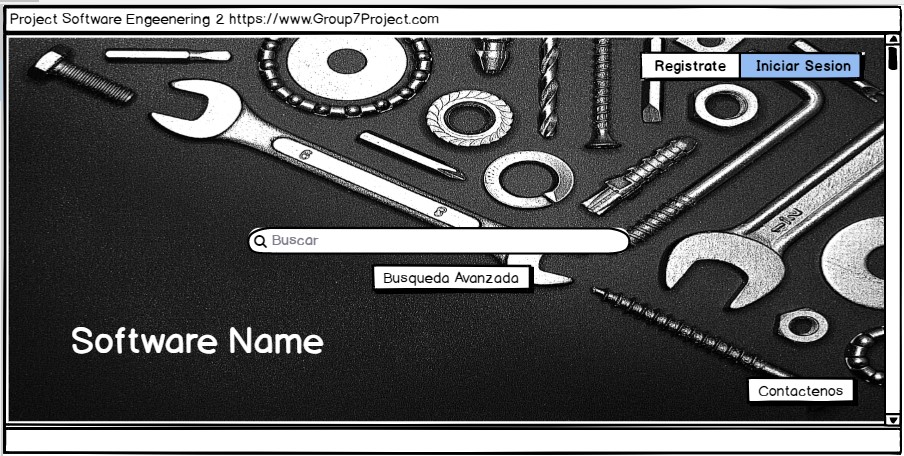
\includegraphics[scale = 0.7]{images/PaginaPrincipal.jpg}
    \caption{Pagina Principal}
    \label{F100}
\end{figure}{}

\begin{figure}[H]
    \centering
    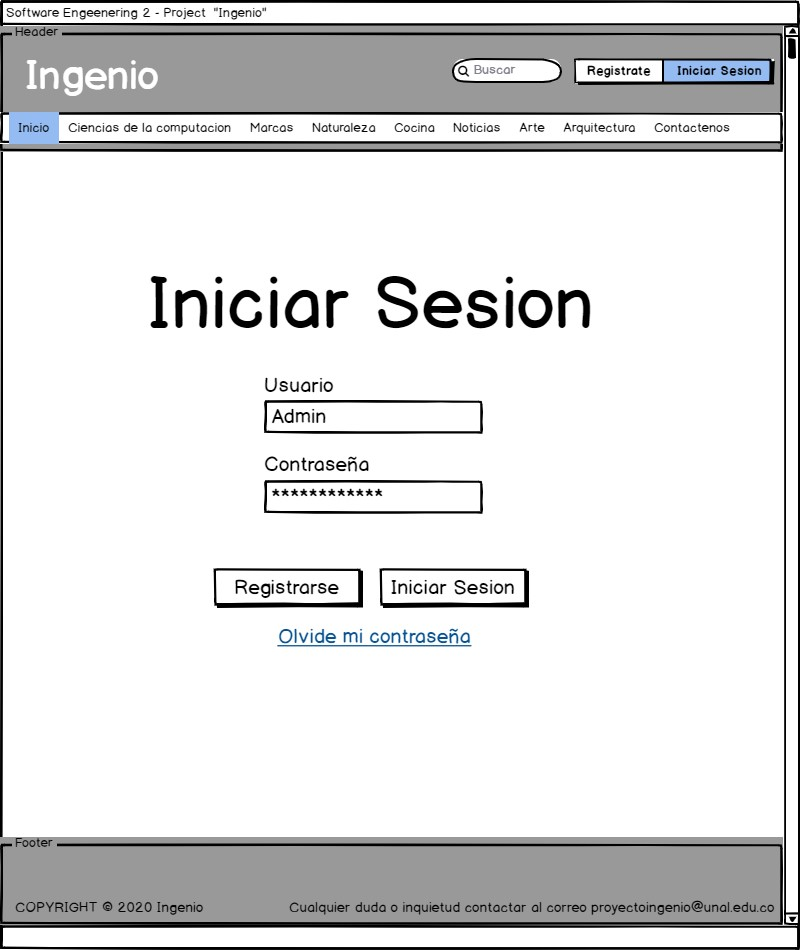
\includegraphics[scale = 0.7]{images/IniciarSesion.jpg}
    \caption{Iniciar Sesión}
    \label{F101}
\end{figure}{}

\begin{figure}[H]
    \centering
    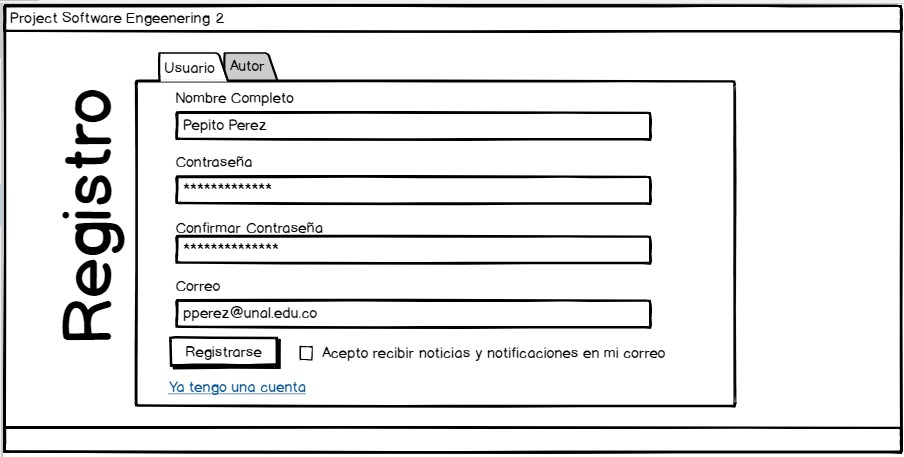
\includegraphics[scale = 0.7]{images/RegistrarseUsuario.jpg}
    \caption{Registrarse Usuario}
    \label{F102}
\end{figure}{}

\begin{figure}[H]
    \centering
    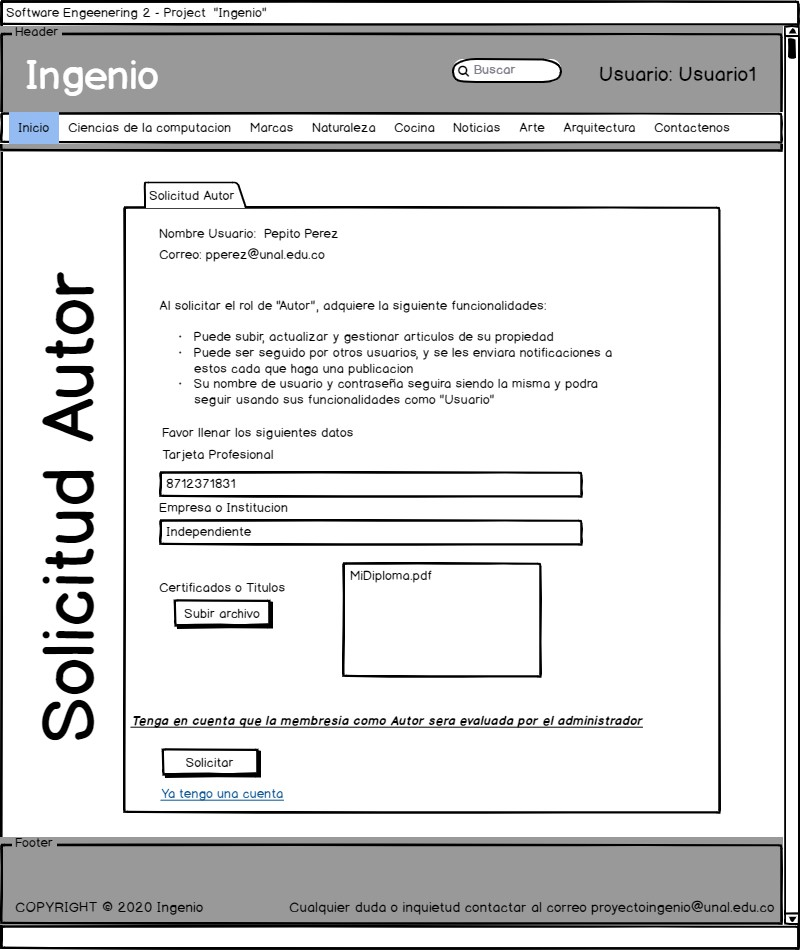
\includegraphics[scale = 0.7]{images/SolicitudAutor.jpg}
    \caption{Solicitud Autor}
    \label{F103}
\end{figure}{}

\begin{figure}[H]
    \centering
    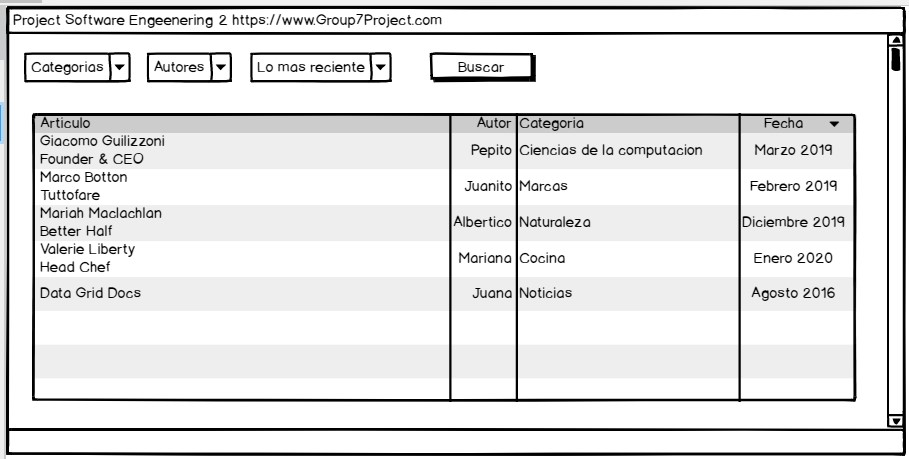
\includegraphics[scale = 0.7]{images/BusquedaAvanzada.jpg}
    \caption{Búsqueda Avanzada}
    \label{F104}
\end{figure}{}

\begin{figure}[H]
    \centering
    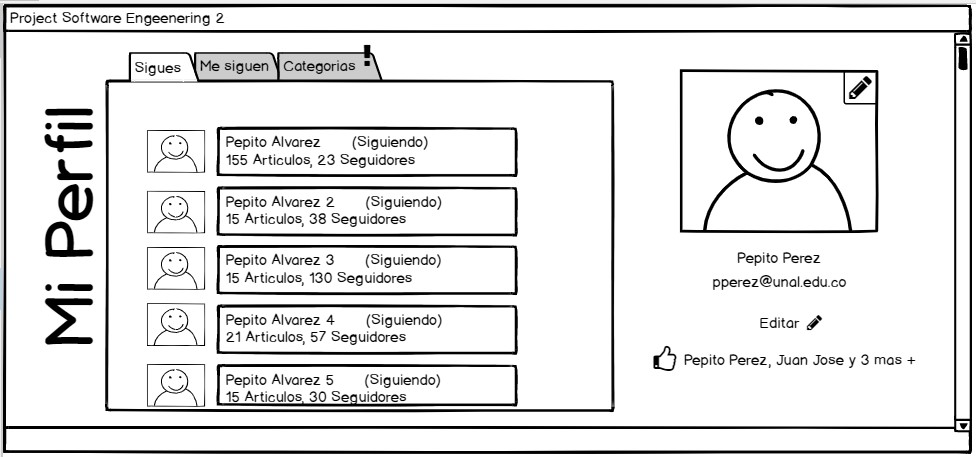
\includegraphics[scale = 0.7]{images/PerfilPropioUsuario.jpg}
    \caption{Perfil Propio Usuario}
    \label{F105}
\end{figure}{}

\begin{figure}[H]
    \centering
    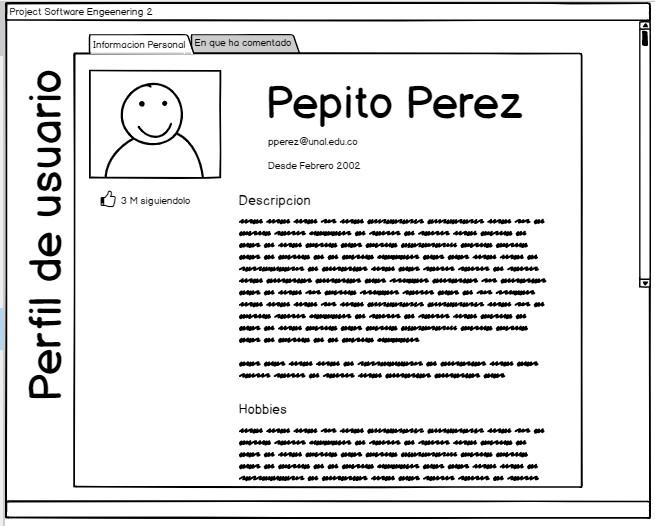
\includegraphics[scale = 0.7]{images/PerfilOtroUsuario.jpg}
    \caption{Perfil Otro Usuario}
    \label{F106}
\end{figure}{}

\begin{figure}[H]
    \centering
    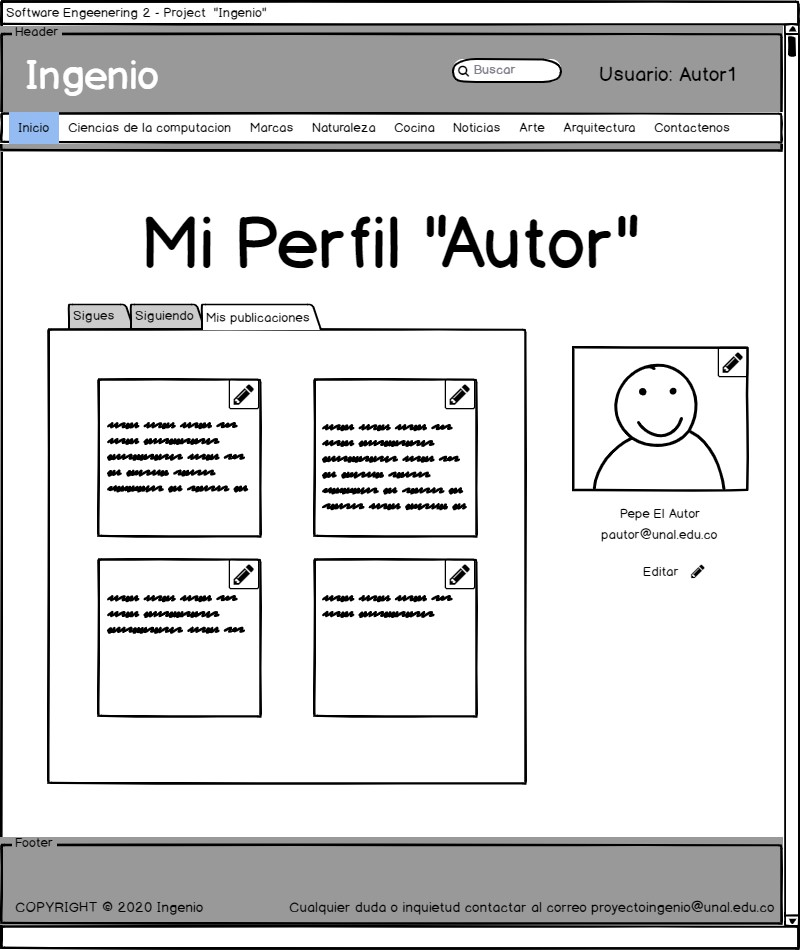
\includegraphics[scale = 0.71]{images/PerfilPropioAutor.jpg}
    \caption{Perfil Propio Autor}
    \label{F107}
\end{figure}{}

\begin{figure}[H]
    \centering
    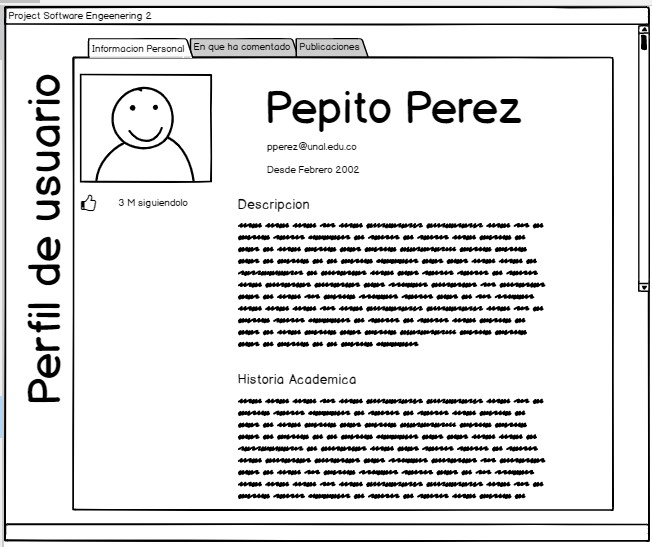
\includegraphics[scale = 0.7]{images/PerfilOtroAutor.jpg}
    \caption{Perfil Otro Autor}
    \label{F108}
\end{figure}{}

\begin{figure}[H]
    \centering
    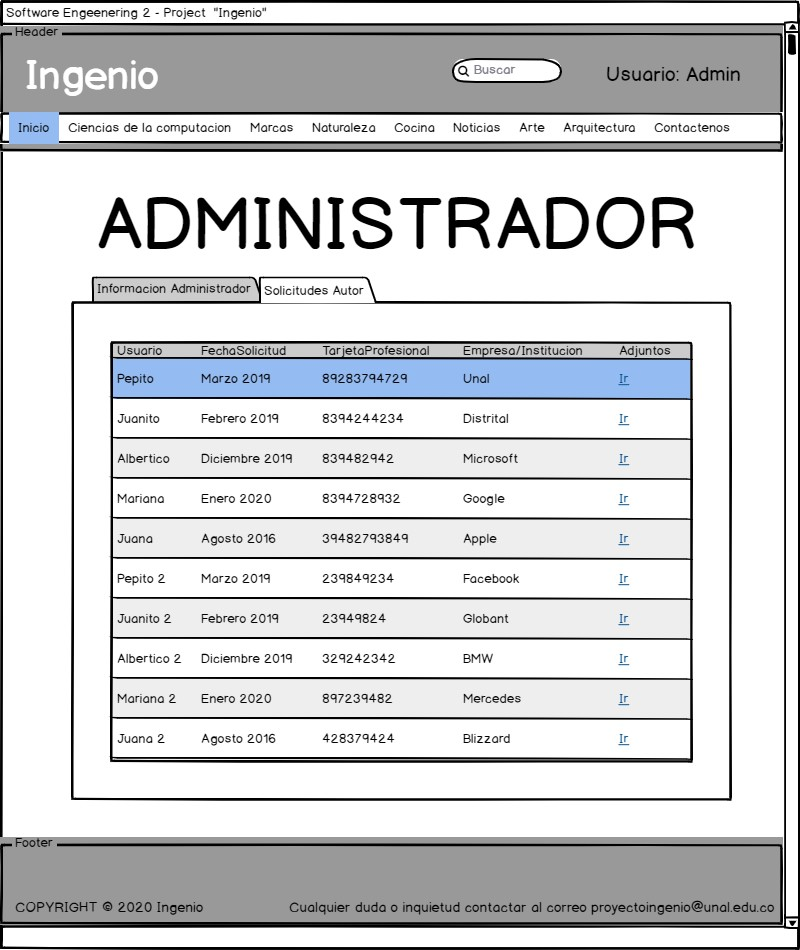
\includegraphics[scale = 0.7]{images/PerfilAdministrador.jpg}
    \caption{Perfil Administrador}
    \label{F109}
\end{figure}{}

\begin{figure}[H]
    \centering
    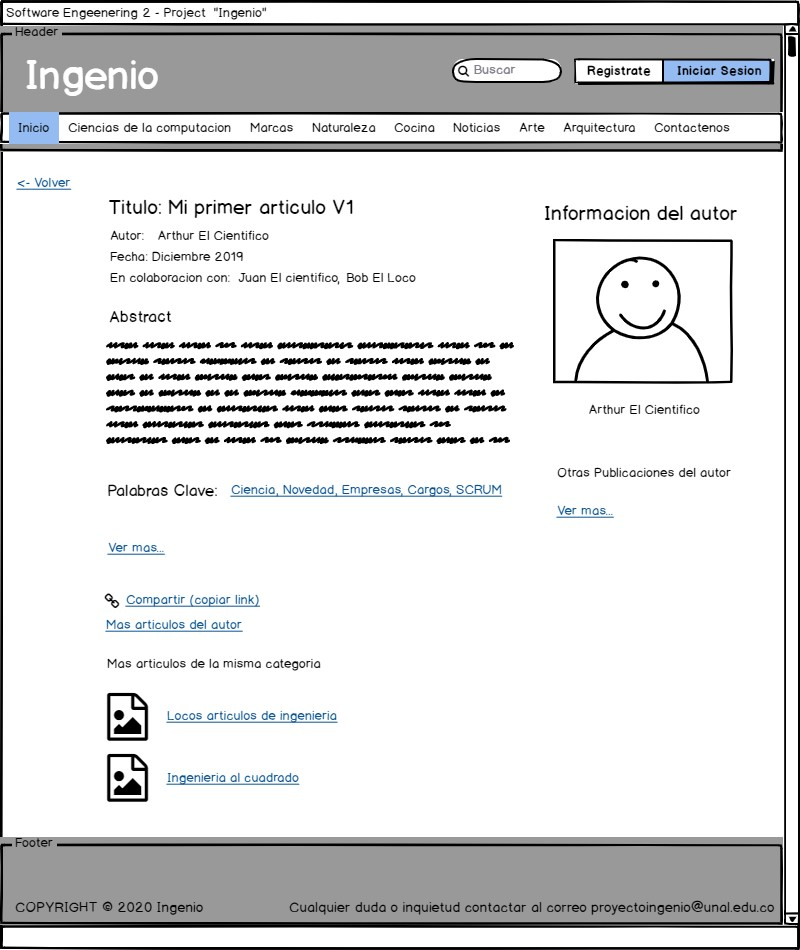
\includegraphics[scale = 0.7]{images/PublicacionVisitante.jpg}
    \caption{Publicación Visitante}
    \label{F110}
\end{figure}{}

\begin{figure}[H]
    \centering
    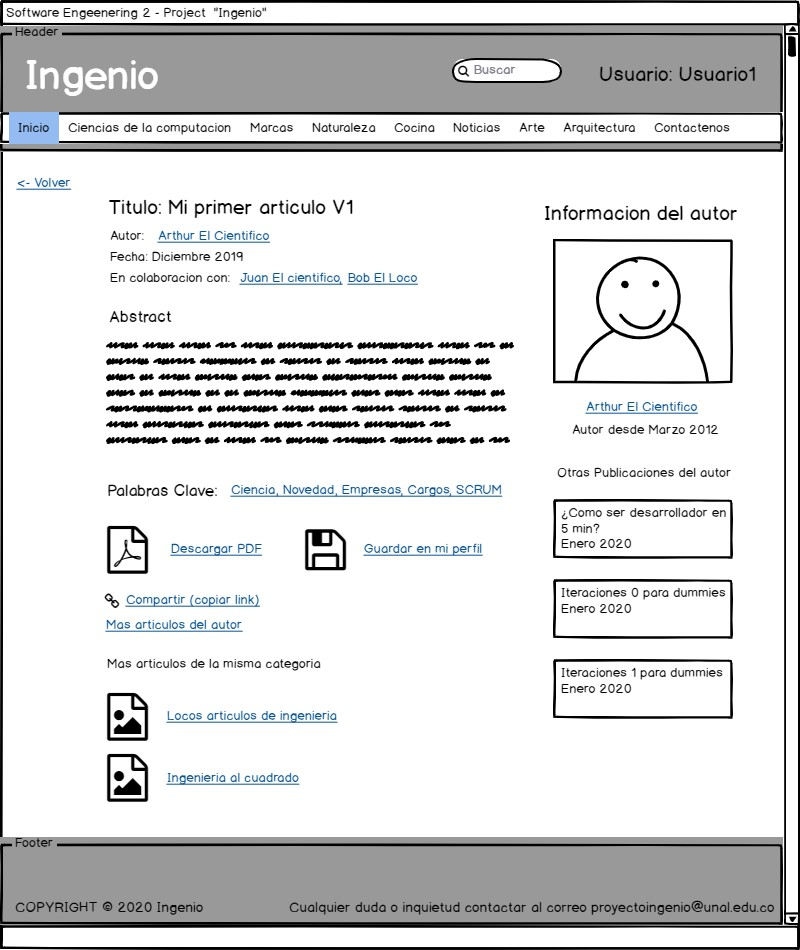
\includegraphics[scale = 0.7]{images/Publicacion.jpg}
    \caption{Publicación}
    \label{F111}
\end{figure}{}

\begin{figure}[H]
    \centering
    
\includegraphics[scale = 0.7]{images/Contactenos.jpg}
    \caption{Contactenos}
    \label{F112}
\end{figure}{}

\begin{landscape}
\section{Modelo Entidad Relación}
    \begin{figure}[H]
        \centering
        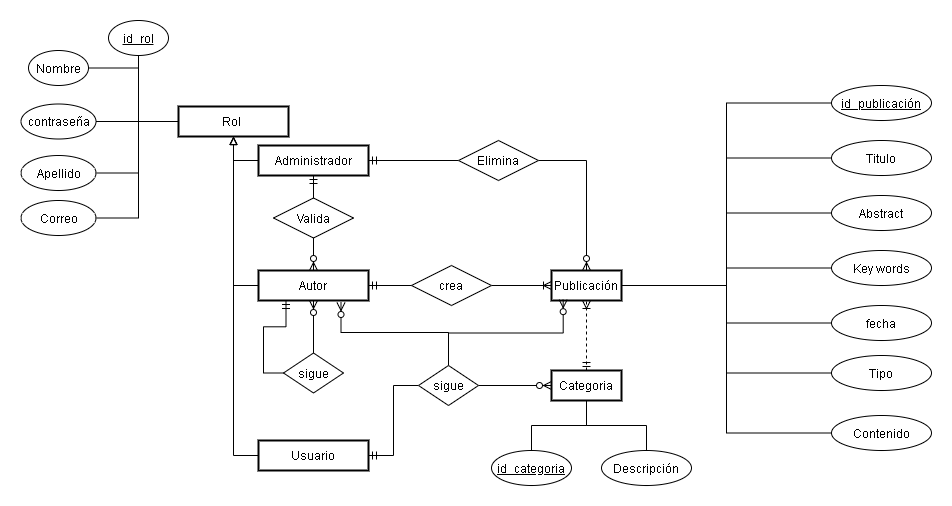
\includegraphics[scale = 0.7]{images/ERD.png}
        \caption{Descripción}
        \label{F13}
    \end{figure}{}

\section{Modelo de Base de Datos}
    \begin{figure}[H]
        \centering
        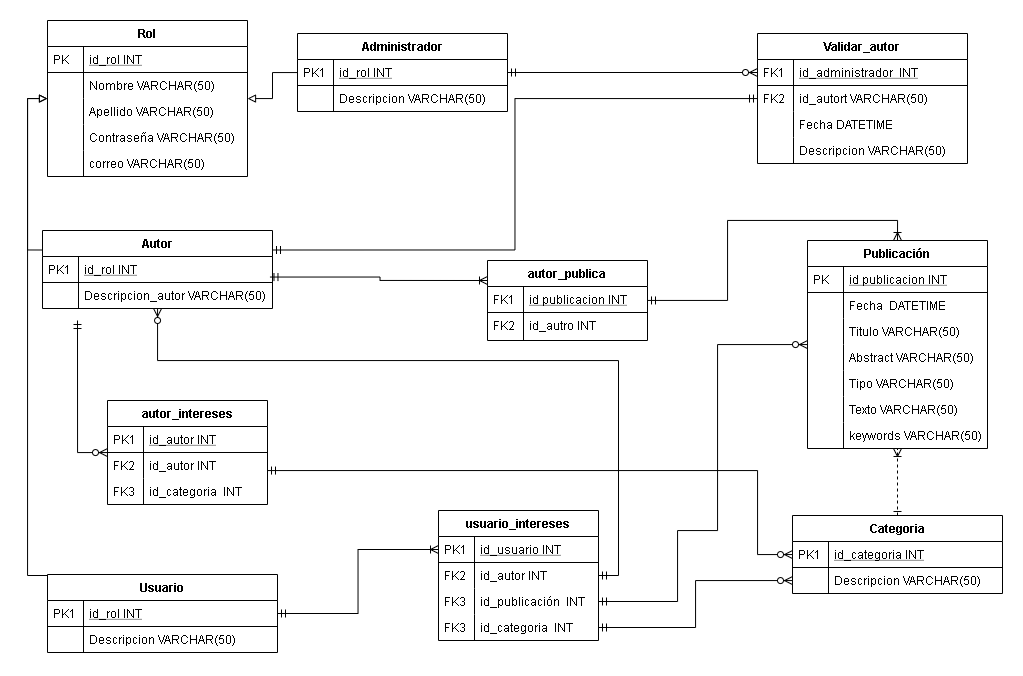
\includegraphics[scale = 0.55]{images/Diagr_BD.png}
        \caption{Descripción}
        \label{F11}
    \end{figure}{}
\end{landscape}

\section{Estimación de Costos}
El tiempo estimado para realizar el proyecto es del 25 de Marzo del 2020 al 25 de Junio
del 2020 (3 meses). \textbf{Por lo tanto todos los gastos se contemplan para este tiempo
estimado}.\\

\textbf{Costos Directos de Personal:}

Los costos directos de personal hacen referencia a las personas contratadas que
colaboran directamente en el proyecto; Scrum Master y 3 desarrolladores.\\

Según la página de búsqueda de empleos “Indeed” \cite{01}, el salario promedio de un
Desarrollador de Software en Colombia es de \$ 2’383.039 COP al mes y para un Scrum
Master es de \$3.942.313 .Tanto el Scrum Master, como los desarrolladores, se encuentran
en últimos semestres de universidad, al momento realizar el proyecto y sus contratos
serán al termino de prestación de servicios. 

% plantilla: copiar y pegar
\begin{table}[H]
    \centering
    \small{
    \begin{tabular}{R{6cm}L{6cm}}
        \textbf{Concepto}   &\textbf{Valor(3 meses)}\\
        \\
        \multicolumn{2}{c}{Scrum master  \dotfill  \$11'826.939} \\
        \multicolumn{2}{c}{Desarrolladores x 3  \dotfill \$21'447.351} \\
        \hline
        \multicolumn{2}{c}{\textbf{Total} \dotfill \$33'274.290} \\
    \end{tabular}
    \label{T04}}
\end{table}{}


\textbf{Costos Indirectos de Personal:}


Los costos indirectos de personal son las personas contratadas que no aportan directamente al proyecto pero que son necesarias para realizar el trabajo.

Se contratara personal de aseo para hacer la limpieza en la oficina dos veces al mes, y se le pagara \$ 30.000 COP / día.

\begin{table}[H]
    \centering
    \small{
    \begin{tabular}{R{6cm}L{6cm}}
        \textbf{Concepto}   &\textbf{Valor(3 meses)}\\
        \\
        \multicolumn{2}{c}{Personal de Aseo  \dotfill  \$180.000} \\
        \hline
        \multicolumn{2}{c}{\textbf{Total} \dotfill \$180.000} \\
    \end{tabular}
    \label{T201}}
\end{table}{}

\textbf{Costos Directos de Material:}

Estos costos son los relacionados a la compra o alquiler de equipos necesarios 
para el desarrollo del software, para este proyecto consideramos el alquiler de 
4 computadores \cite{02} por un valor mensual de \$220.000 COP / cada uno, además se consideran 
el consumo de internet y energía eléctrica en el lugar de desarrollo, estos corresponden a un valor de \$110.000 COP/mensual de servicio 
de energía eléctrica y \$103.000 COP / mensual por servicio de internet, también se contempla la compra de mueblería a usar, que consta de 4 escritorios y 4 sillas, por valor de \$2'000.000 COP.

\begin{table}[H]
    \centering
    \small{
    \begin{tabular}{R{6cm}L{6cm}}
        \textbf{Concepto}   &\textbf{Valor(3 meses)}\\
        \\
        \multicolumn{2}{c}{Alquiler de equipos x 4  \dotfill  \$2'640.000} \\
        \multicolumn{2}{c}{Servicio de energía eléctrica\dotfill  \$330.000} \\
        \multicolumn{2}{c}{Servicio de internet \dotfill \$309.000} \\
        \multicolumn{2}{c}{Compra Mueblería \dotfill \$2'000.000} \\
        \hline
        \multicolumn{2}{c}{\textbf{Total} \dotfill \$5'279.000} \\
    \end{tabular}
    \label{T03}}
\end{table}{}

\textbf{Costos Indirectos de Material:}

Estos costos son los no relacionados directamente con el proyecto, pero necesarios en el ambiente de trabajo.
Tales como, recibo de agua por un valor mensual de \$120.000 COP, además implementos de aseo que corresponden a un valor de \$150.000 COP/mensual y gastos varios o de papelería por \$50.000 COP / mensual.

\begin{table}[H]
    \centering
    \small{
    \begin{tabular}{R{6cm}L{6cm}}
        \textbf{Concepto}   &\textbf{Valor(3 meses)}\\
        \\
        \multicolumn{2}{c}{Servicio de agua \dotfill  \$360.000} \\
        \multicolumn{2}{c}{Implementos de aseo 
        \dotfill  \$450.000} \\
        \multicolumn{2}{c}{Papelería y varios
        \dotfill \$150.000} \\
        \hline
        \multicolumn{2}{c}{\textbf{Total} \dotfill \$960.000} \\
    \end{tabular}
    \label{T203}}
\end{table}{}

\textbf{Total de Costos:}

En esta sección se encuentra el resumen de todos los costos del proyecto, y el valor final a cobrar.

\begin{table}[H]
    \centering
    \small{
    \begin{tabular}{R{6cm}L{6cm}}
        \textbf{Concepto}   &\textbf{Valor(3 meses)}\\
        \\
        \multicolumn{2}{c}{Costos directos personal  \dotfill  \$33'274.290} \\
        \multicolumn{2}{c}{Costos indirectos personal  \dotfill  \$180.000} \\
        \multicolumn{2}{c}{Costos directos de material \dotfill \$5'279.000} \\
        \multicolumn{2}{c}{Costos indirectos de material \dotfill \$960.000} \\
        \hline
        \multicolumn{2}{c}{\textbf{Total (antes de instalación)} \dotfill \$39'693.290} \\
        \multicolumn{2}{c}{Instalación \dotfill \$500.000} \\
        \hline
        \multicolumn{2}{c}{\textbf{Total (antes de ganancia esperada)} \dotfill \$40'193.290} \\
        \multicolumn{2}{c}{Ganancia esperada (20\%) \dotfill \$8'038.658} \\
        \hline
        \multicolumn{2}{c}{\textbf{Total (Precio mínimo)} \dotfill \$48'231.948} \\
        \multicolumn{2}{c}{Ajuste Final \dotfill - \$231.948} \\
        \hline
        \multicolumn{2}{c}{\textbf{Total Esfuerzo Nominal} \dotfill \$48'000.000} \\
        \multicolumn{2}{c}{Esfuerzo de sobrecarga (50\%) \dotfill - \$24'000.000} \\
        \hline
        \multicolumn{2}{c}{\textbf{Costo Total} \dotfill \$72'000.000} \\
    \end{tabular}
    \label{T205}}
\end{table}{}

Se estima un valor total \$72'000.000 COP por el costo total del proyecto.


\section{Análisis de riesgos}


\begin{table}[H]
    \centering
    \small{
    \begin{tabular}{|M{1cm}|M{3cm}|M{8cm}|}
        \hline
        \textbf{Valor}  &\textbf{Tipo}   &\textbf{Definición}\\
        \hline 
        \multirow{1}{1cm}{\centering 1}    
            & \multirow{1}{3cm}{\centering Técnico}
            & Criterio      \\
        \hline
        \multirow{1}{1cm}{\centering 2}
            & \multirow{1}{3cm}{\centering Organizacional}
            & Criterio      \\
        \hline
        \multirow{1}{1cm}{\centering 3}
            & \multirow{1}{3cm}{\centering Cronograma}
            & Criterio      \\
        \hline
        \multirow{1}{1cm}{\centering 4}
            & \multirow{1}{3cm}{\centering Externo}
            & Criterio      \\
        \hline
        \multirow{1}{1cm}{\centering 5}
            & \multirow{1}{3cm}{\centering Gerencial}
            & Criterio      \\
        \hline
    \end{tabular}
    \caption{Tipos de riesgo}
    \label{Riesgo}}
\end{table}{}


\begin{table}[H]
    \centering
    \small{
    \begin{tabular}{|M{1cm}|M{2cm}|M{8cm}|}
        \hline
        \textbf{Valor}   &\textbf{Significado}   &\textbf{Criterio}\\
        \hline 
        \multirow{1}{1cm}{\centering 1}    
            &\multirow{1}{2cm}{\centering Muy bajo}
            & Criterio      \\
        \hline
        \multirow{1}{1cm}{\centering 2}    
            &\multirow{1}{2cm}{\centering Bajo}
            & Criterio      \\
        \hline
        \multirow{1}{1cm}{\centering 3}    
            &\multirow{1}{2cm}{\centering Moderado}
            & Criterio      \\
        \hline
        \multirow{1}{1cm}{\centering 4}    
            &\multirow{1}{2cm}{\centering Alto}
            & Criterio      \\
        \hline
        \multirow{1}{1cm}{\centering 5}    
            &\multirow{1}{2cm}{\centering Muy alto}
            & Criterio      \\
        \hline
    \end{tabular}
    \caption{Niveles de Impacto}
    \label{Nimpacto}}
\end{table}{}

\begin{table}[H]
    \centering
    \small{
    \begin{tabular}{|M{3.5cm}|M{1cm}|M{1.5cm}|M{2.5cm}|M{4cm}|}
         \hline
            \textbf{Riesgo} & \textbf{Tipo} &\textbf{Impacto}
            & \textbf{Probabilidad} & \textbf{Plan de acción}\\
         \hline
         \multirow{1}{3cm}{\centering Ries}
             & \multirow{1}{1cm}{\centering 1}
             & \multirow{1}{1.5cm}{\centering 5}
             & \multirow{1}{2.5cm}{\centering 50\%}
             &  Descrip     \\
        \hline
         \multirow{1}{3cm}{\centering Ries}
             & \multirow{1}{1cm}{\centering 1}
             & \multirow{1}{1.5cm}{\centering 5}
             & \multirow{1}{2.5cm}{\centering 50\%}
             &  Descrip     \\
        \hline
         \multirow{1}{3cm}{\centering Ries}
             & \multirow{1}{1cm}{\centering 1}
             & \multirow{1}{1.5cm}{\centering 5}
             & \multirow{1}{2.5cm}{\centering 50\%}
             &  Descrip     \\
             
        \hline
         \multirow{1}{3cm}{\centering Ries}
             & \multirow{1}{1cm}{\centering 1}
             & \multirow{1}{1.5cm}{\centering 5}
             & \multirow{1}{2.5cm}{\centering 50\%}
             &  Descrip     \\
        \hline
         \multirow{1}{3cm}{\centering Ries}
             & \multirow{1}{1cm}{\centering 1}
             & \multirow{1}{1.5cm}{\centering 5}
             & \multirow{1}{2.5cm}{\centering 50\%}
             &  Descrip     \\
        \hline
         \multirow{1}{3cm}{\centering Ries}
             & \multirow{1}{1cm}{\centering 1}
             & \multirow{1}{1.5cm}{\centering 5}
             & \multirow{1}{2.5cm}{\centering 50\%}
             &  Descrip     \\
        \hline
         \multirow{1}{3cm}{\centering Ries}
             & \multirow{1}{1cm}{\centering 1}
             & \multirow{1}{1.5cm}{\centering 5}
             & \multirow{1}{2.5cm}{\centering 50\%}
             &  Descrip     \\
        \hline
    \end{tabular}
    \caption{Riesgos de desarrollo}
    \label{riesgos}}
\end{table}{}


\begin{thebibliography}{50}
\bibitem{01} Indeed Salarios. Disponible en:\url{https://co.indeed.com/salaries/desarrollador-de-software-Salaries}
\bibitem{02} Renta sistemas. Disponible en:\url{https://www.rentasistemas.com/}


\end{thebibliography}{}

\end{document}{}

